\chapter{Reproducing Kernel Hilbert spaces (RKHS) for Differential TD Learning}
\label{ch:rkhs} \anandspm{Can you read this section till the beginning of 3.1? }
In \Chapter{ch:diff_td}, the standard LSTD algorithm was reviewed and two versions of the differential TD learning algorithm were presented. An important step in all these algorithms is the selection of a suitable approximating function class, characterized by  a linear or nonlinear parameterization. It is noted in \cite{ctcn} that any insight about the true value function can aid in this step. For example, if the value function is known to obey certain properties, say convexity, then the basis functions chosen can also be convex.  In certain examples, the value function at a state can provide useful information about the values at ``neighboring'' states. In the case of stochastic optimal control, the fluid value functions provide a natural starting point to approximate the solution to the average-cost value function. However, such choices are heavily problem-dependent and no standard methods exist. In most traditional examples of TD learning, a predetermined set of basis functions is used to define the function class. This limits the learning capability in two ways:
\begin{romannum}
	\item The chosen function class may not be rich enough to give a good approximation of the value function.
	\item The approximation algorithms discussed in this dissertation are based on Monte Carlo methods with finite sample size. A predetermined set of basis functions will not be able to exploit information about the distribution of these samples in the state space.  
\end{romannum}
Hence, it is a better idea to choose a function class that adapts dynamically to suit the problem and the sample distribution. Kernel methods provide an alternative approach to basis selection. 

This chapter aims to adapt the $\gradTD$-L algorithm proposed in \Chapter{ch:diff_td} in a reproducing kernel Hilbert space (RKHS) setting.  The remainder of this chapter is organized as follows - In \Section{s:rkhs_basics}, a very concise introduction to kernel functions and the RKHS theory is provided. A more detailed discussion of its properties including Mercer's theorem can be found in \Appendix{a:mercers_theorem}. Gaussian kernels have found wide acceptance in machine learning and function approximation and some of the useful properties of the RKHS induced by the Gaussian kernel is discussed in \Appendix{a:gaussian_rkhs}. Function approximation problems arising in machine learning are usually cast in the form of a regularized empirical risk minimization (ERM) problem - a brief introduction is provided in \Section{s:erm}. Obtaining solutions to such problems are made possible via the classical representer theorem. The theorem is stated in \ref{s:erm_rkhs} and the proof is provided in \Appendix{a:rep_theorem}. In \Section{s:erm}, the minimum-norm problem in $L^2(\pr)$ \eqref{e:diff_td_gradTD_norm_error} of approximating the gradient of the solution to Poisson's equation is reformulated as an equivalent ERM problem to apply the RKHS machinery. As the ERM formulated consists of gradient terms, a generalized  version of the representer theorem is required to obtain the optimal solution.  A simplified sub-optimal solution that lies on a subspace of the original RKHS is also presented. We provide a short review of an error analysis approach for a generic least squares regression problem in an RKHS in \Appendix{a:bousquet}. Error analysis for ERMs with loss functions having gradient terms is a topic for future research. \anandspm{is this statement about error analysis okay?}

\section{RKHS Basics}
\label{s:rkhs_basics}
Kernel methods have been quite well-studied for over five decades now. They provide a flexible and mathematically-elegant framework for a range of estimation problems by relating them to a function reconstruction problem in a higher dimensional feature space. By controlling the features of this space, the properties of the candidate functions can also be implicitly controlled. \anand{From Bhujwalla's thesis, need to rephrase}The mathematical properties of kernel functions were first investigated by Moore \cite{moo1916} and Mercer \cite{merrus09} in the early twentieth century. Although initial applications were in time series analysis, detection, filtering and prediction problems, more recently they have been found to be incredibly useful in machine learning \cite{wah90}, especially after the advent of support vector machines (SVM) for classification and regression problems \cite{corvap95, drucburkaufsmovap97}. In this dissertation, the goal is to employ kernel methods as an alternative to finite dimensional basis selection for the $\gradTD$-L learning algorithm. 

\subsection{Reproducing Kernels} 
Before defining an RKHS, a positive definite kernel needs to be defined. A function $\Kern : \state \times \state \to \Re$ which for all $N \in \mathbb{N}$ and all $x^1,x^2,\cdots,x^N \in \state$ gives rise to a positive definite Gram matrix is a called a positive definite kernel. That is, 
\begin{equation}
\sum_{i=1}^N \sum_{j=1}^N \alpha_i \alpha_j \Kern(x^i,x^j) \geq 0, \qquad \forall \alpha_i \in \Re, \, \forall x^i \in \state 
\end{equation}
Let us consider a function $f$ which is a linear combination of the form,
\begin{equation}
f(\cdot) = \sum_{i=1}^N \alpha_i \Kern(x^i, \cdot),
\label{e:rkhs_f_rkhs}
\end{equation}
where $N \in \mathbb{N}, \alpha_i \in \Re, \{ x^i \in \state: 1\leq i \leq N \}$ are arbitrary. Let $\clH^0$ denote the vector space (pre-Hilbert space) spanned by all functions $f$ of this form. Evidently, the function $g$ defined as,  
\begin{equation}
g(\cdot) = \sum_{j=1}^M \rkhsparam_j \Kern(x^j, \cdot),
\label{e:rkhs_g_rkhs}
\end{equation}
where each $\rkhsparam_i \in \Re$ and $\{x^j\}_1^M$ are arbitrary points, also belongs to this vector space.  An inner product of functions $f,g \in \clH^0$ is defined as,
\begin{equation}
\langle f,\, g \rangle \eqdef \sum_{i=1}^N \sum_{j=1}^M \alpha_i \rkhsparam_j \Kern(x^i, x^j).
\label{e:rkhs_inner_product}
\end{equation}
It is interesting to note that the inner product is independent of the expansions used for $f$ and $g$, i.e.
\begin{equation}
\langle f, g \rangle = \sum_{i=1}^N \alpha_i g(x^i) = \sum_{j=1}^N \rkhsparam_j f(x^j)
\end{equation}
The reproducing property of the kernel $\Kern$ follows from the definition of the inner product \eqref{e:rkhs_inner_product},
\begin{equation}
\langle \Kern(x,\cdot), f(\cdot)\rangle = f(x) \qquad \forall x \in \state, \forall f \in \clH^0.
\label{e:rkhs_rep_property}
\end{equation}
Owing to this property, the kernel function $\Kern$ is called the reproducing kernel. It is also called the evaluation functional as it evaluates the function $f$ at a point $x$. The symmetry of the kernel $\Kern$ guarantees that the inner product definition satisfies the commutative property, i.e. if $\Kern_x = \Kern(x, \cdot)$ we have,
\begin{equation}
\langle \Kern_x, \Kern_{x'} \rangle =  \Kern(x,x') = \Kern(x',x) =  \langle \Kern_{x'}, \Kern_x \rangle. 
\end{equation}
The space obtained by the completion of functions of the form $f$ defined in \eqref{e:rkhs_f_rkhs}, that are endowed with the inner product defined in \eqref{e:rkhs_inner_product} (denoted as $\langle \cdot, \cdot \rangle_{\clH}$ here onward to distinguish from the normal dot product definition) yields a Hilbert space $\clH$, called the reproducing kernel Hilbert space (RKHS). The corresponding norm is defined as $\|f\|_\clH \eqdef \sqrt{\langle f, f \rangle_\clH}$. 

The Moore-Aronszajn theorem states that every symmetric, positive definite kernel $\Kern : \state \times \state \to \Re$ defines an RKHS $\clH$ for which $\Kern$ is the reproducing kernel. A Hilbert function space $\clH$ that has a reproducing kernel $\Kern$ is always an RKHS and conversely, every RKHS has a (unique) reproducing kernel. While all RKHS are Hilbert spaces, the converse is not true. For example, the space of square-integrable $L^2$ functions is a Hilbert space, but not an RKHS. 

The reproducing kernel Hilbert spaces have the remarkable property that norm convergence implies pointwise convergence. 
For any function $f\in\clH$ and $\{f_n\}\subset \clH$ be a sequence with $\|f_n - f\|_\clH \to 0$ for $n \to \infty$, then for all $x \in \state$, we have,
\begin{equation}
\lim_{n\to\infty} f_n(x) = \lim_{n \to \infty} \langle \Kern_x,  f_n \rangle_\clH = \langle \Kern_x, f \rangle_\clH = f(x)
\end{equation}
If $\Kern$ is a continuous, symmetric and positive definite kernel satisfying, 
\begin{equation}
\kappa = \sup_{x \in \state} \sqrt{\Kern(x,x)} < \infty,
\label{e:rkhs_kappa}
\end{equation}
then, \Prop{prop:RKHS_bounded} holds. Additionally, if $K$ is continuous, then every function in $\clH$ is continuous. 
\begin{proposition}
\label{prop:RKHS_bounded}
	If the kernel $\Kern$ is uniformly bounded by \eqref{e:rkhs_kappa}, then any $f \in \clH$ is also bounded. 
\end{proposition}
\begin{proof}
	If $f \in \clH$, for all $x \in \state$,
	\begin{equation}
	\begin{aligned}
	|f(x)| &= |\langle \Kern(x,\cdot), f \rangle_\clH| \\
	& \leq \|\Kern(x,\cdot)\|_\clH \|f\|_\clH, \qquad{\text{(By Cauchy-Schwarz inequality)}}\\ 
	& \leq \kappa \|f\|_\clH
	\end{aligned}
	\end{equation}
	As the above inequality holds for all $x \in \state$, 
	\begin{equation}
	\|f\|_\infty := \max_{x\in \state}|f(x)| \leq \kappa \|f\|_\clH
	\end{equation}
\end{proof}


The RKHS also has a feature map representation. Let $\featuremap: \state \to \Re^\state$ be a feature map that maps each point from $\state$ into a function mapping $\state$ to $\Re$, i.e. $\Re^\state \eqdef \{f: \state \to \Re \}$. The map $\featuremap$ is non-unique, but a canonical feature map exists and is given by $\featuremap(x)  =  \Kern(x,\cdot)$, %\notes{needs citation}
\begin{equation}
\begin{aligned}
\Kern(x,x') &= \langle \featuremap(x), \featuremap(x')\rangle \\
& = \langle \Kern_x, \Kern_{x'} \rangle_\clH
\end{aligned}
\label{e:rkhs_feature_map}
\end{equation}

%\subsection{Orthonormal Basis Functions and Mercer's Theorem} %\anand{Mercer's theorem?}
%Given an RKHS $\clH$, it is useful to understand the set of functions that belong to the Hilbert space. This can be studied using Mercer's theorem \cite{merrus09}. Mercer's theorem forms the connection between the theory of reproducing kernels and integral operators. 
%Consider the integral operator (Hilbert-Schmidt operator) $L_K:L^2_\measure(x) \to L^2_\measure(x)$ defined by,
%\begin{equation}
%(L_K f)(x) = \int_\state \Kern(x,t) f(t) d\measure(t)
%\end{equation}
%where $\measure$ is a finite Borel measure and $\state$ is a compact set.
%The linear map $L_K^{1/2}$, which denotes the square root of $L_K$ is a Hilbert isomorphism between $L^2_{\measure}(\state)$ and $\clH$ as illustrated in \Fig{fig:rkhs_isomorphism}. 
%
%\begin{figure}[htbp]
%	\centering
%	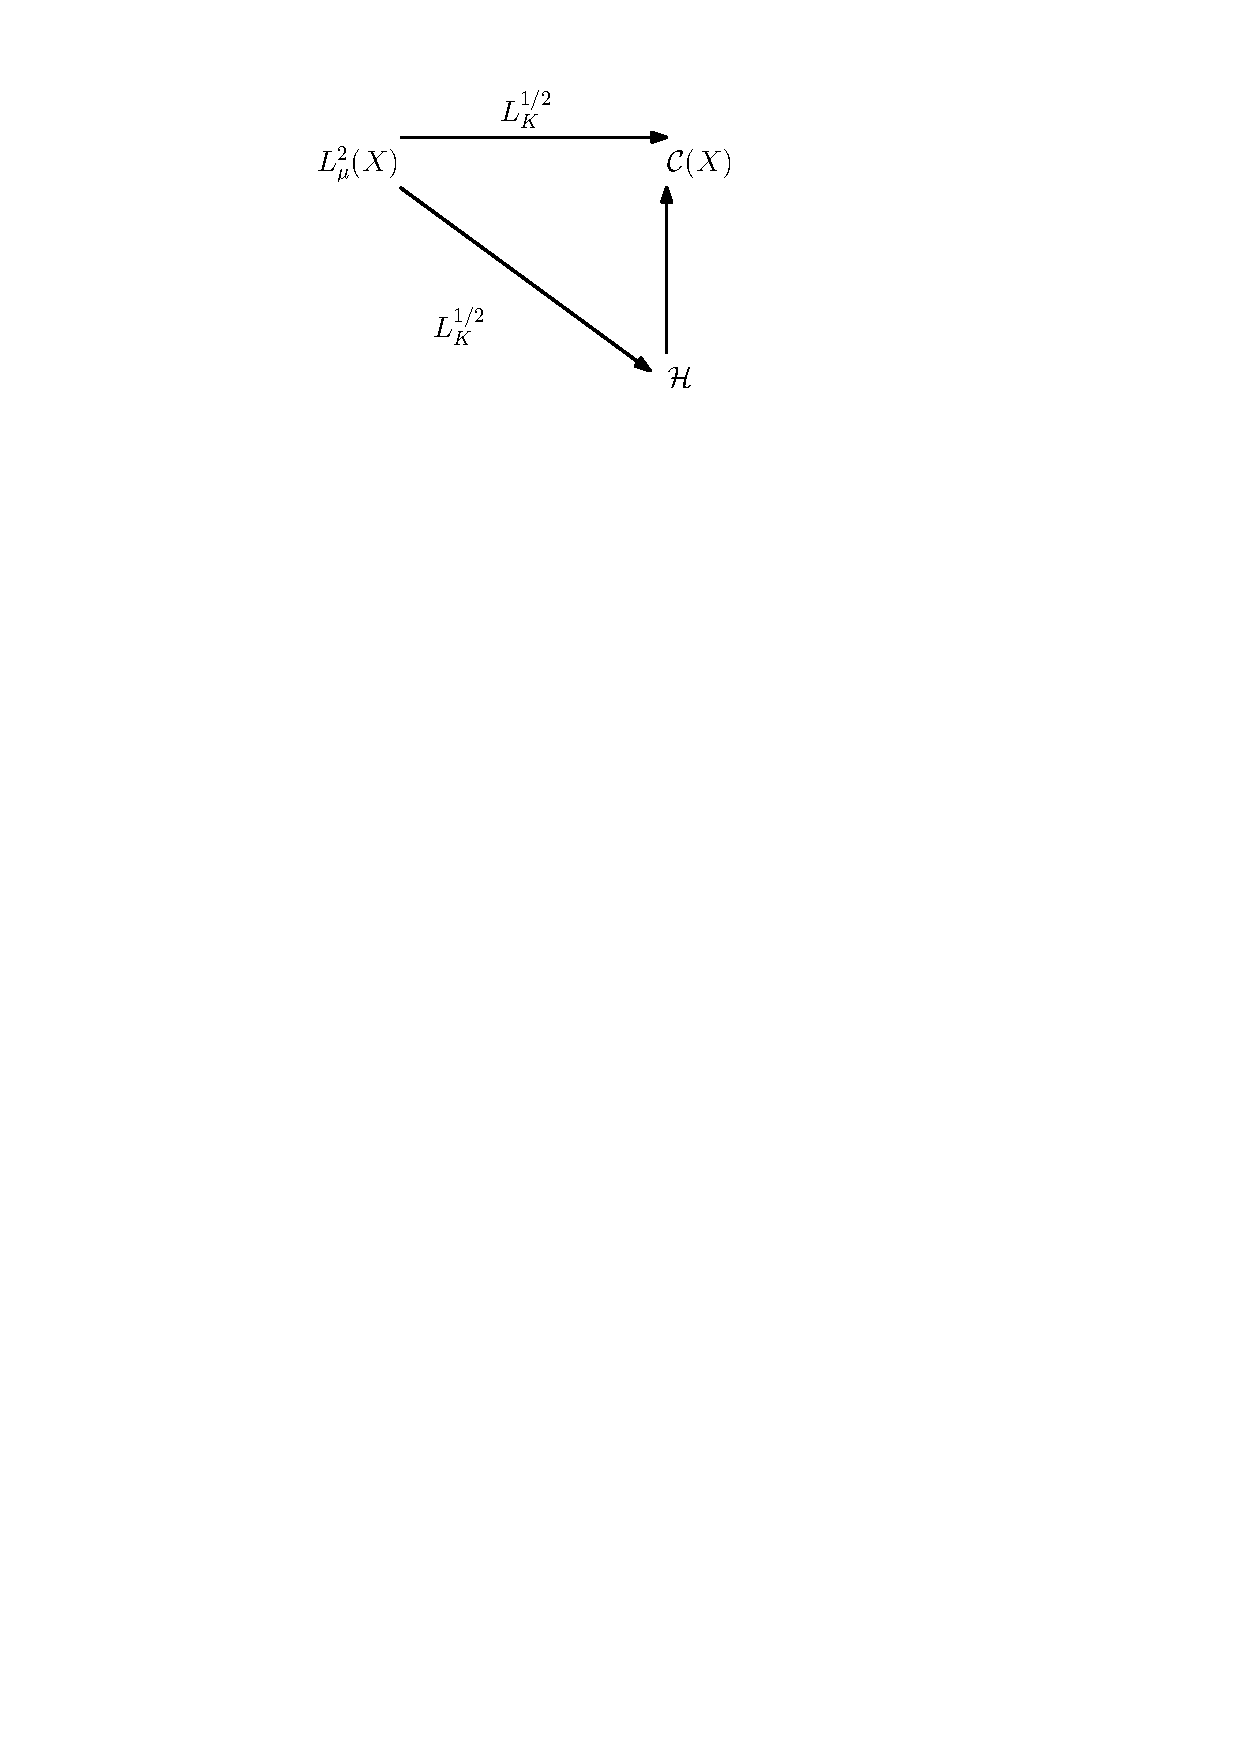
\includegraphics[width=3in]{images/Chap3_RKHS_isomorphism}
%	\caption{Diagram illustrating the isomorphic transformations between $\clH$ and $L^2_\measure$.}
%	\label{fig:rkhs_isomorphism}
%\end{figure}
%
%% $L_{K,C}$ emphasizes that the target is $\mathcal{C}(\state)$ and $I_K$ denotes the inclusion. If $\Kern$ is $\mathcal{C}^\infty$, then $I_K$ is compact. \anand{Gaussian kernel is $\mathcal{C}^\infty$}
% $L_K$ is a self-adjoint, compact operator with eigenvalues $\reg_1 \geq \reg_2 \geq \cdots \geq 0$, with the corresponding normalized eigenfunctions $\{\phi_n\}_{n=1}^\infty$ forming an orthonormal basis for $L^2_\measure(\state)$. Mercer's theorem states that 
%\begin{equation}
%\Kern(x,x') = \sum_{n=1}^\infty \reg_n \phi_n(x) \phi_n(x'),
%\end{equation}
%where the series converges absolutely for each $x,x' \in \state$. The set $\{\sqrt{\reg_n}\phi_n\}_{n=1}^\infty$ forms an orthonormal basis for $\clH$. However, finding an eigenfunction feature representation for a kernel is challenging, except in special cases. 

%\section{Properties of the Gaussian Kernel -  RKHS}
%\label{s:gaussian_rkhs}
%
%Of the many kernels being used, Gaussian kernel is the most widely used and often gives the best performance \cite{min10}. The study of the properties of the Gaussan kernel has received a lot of attention \cite{stehussco06, min10,micchaxuzha06}. The Gaussian kernel is a translation-invariant kernel given by,
%\begin{equation}
%\Kern_{\epsy}(x,x') := \exp(-\|x - x'\|^2/ 4\epsy) \qquad \forall x,x' \in \state,
%\end{equation}
%where $\epsy$ is a parameter that defines the width of the kernel. An illustration of the Gaussian kernel for $\epsy = 0.125$ and the corresponding Fourier transform is given in \Fig{fig:gaussian_kernel}. It may be seen that the Fourier transform decays exponentially fast for large values of $\omega$. The lack of high frequency components in the Gaussian kernel indicates that the functions belonging to the induced RKHS are smooth.  
%\begin{figure}[htbp]
%	\centering
%	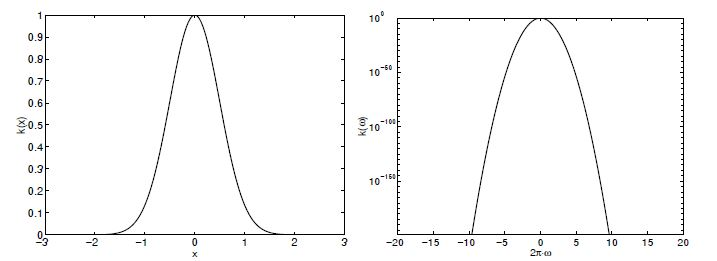
\includegraphics[width=6in]{images/Chap3_Gaussian_kernel}
%	\caption{Gaussian kernel with $\epsy = 0.125$ and its Fourier transform \cite{schsmo01}.}
%	\label{fig:gaussian_kernel}
%\end{figure}
%
%Steinwart et al. in \cite{stehussco06} tries to answer questions like - which functions are contained in the RKHS induced by the Gaussian kernel, how the corresponding norms can be computed, and how the RKHS of different widths correlate to each other. 
%In particular, RKHS of Gaussian kernels always have countable orthonormal bases. Theorem 3 of the paper gives the orthonormal basis functions for $\clH$ defined by the Gaussian kernel $\Kern_\epsy$. It states that for $\epsy >0$ and $n \in \mathbb{N}_0 := \mathbb{N} \cup \{0\}$, the sequence of functions $\{\phi_n : \Re \to \Re\}$ defined by,
%\begin{equation}
%\phi_n(x) := \sqrt{\frac{1}{(2\epsy)^n n!}}x_n \exp(-x^2/4\epsy).
%\end{equation}
%is an orthonormal basis for $\clH$.
%
%Minh in \cite{min10} gives several properties of the RKHS induced by Gaussian kernels. Theorem 1 of the paper states that the RKHS $\clH$ induced by the standard Gaussian kernel is infinite dimensional, i.e. dim($\clH$) = $\infty$ and 
%\begin{equation}
%\clH := \Bigl\{ f = \exp(-x^2/4\epsy) \sum_{n=0}^\infty w_n x_n: \|f\|^2_\clH = \sum_{k=0}^\infty (2\epsy)^k k! \sum_{n=0}^k w_n^2 <\infty \Bigr\}
%\end{equation}
%Some of the salient properties of the Gaussian kernel RKHS are summarized below: 
%\begin{enumerate}
%	\item $\clH$ induced by the standard Gaussian kernel does not contain any polynomial on $\state$, including the non-zero constant function. 
%	
%	\item If $\state$ is compact, $\clH$ induced by the Gaussian kernel is dense in the space of $\mathcal{C}(\state)$ of continuous functions on $\state$.
%	This means that given a continuous function $h(x)$, for all $\varepsilon >0$, we can find a function $g(x) \in \clH$ such that 
%	\begin{equation}
%	\|h(x) - g(x)\|_\infty \leq \epsy \qquad \forall x \in \state
%	\end{equation} 
%	\item Let $\Kern_{\epsy}(x,x') = \exp(-\frac{\|x-x'\|^2}{4\epsy})$. The Hilbert space $\clH_\epsy$ induced by $\Kern_\epsy$ on $\state$ contains the function $\exp(-\frac{c \|x\|^2} {4 \epsy})$ if and only if $0<c <2$. For example, $\exp(-\frac{\|x\|^2}{2 \epsy}) \in \clH_{\epsy/2}$, but  $\exp(-\frac{\|x\|^2}{2 \epsy}) \notin \clH_{\epsy}$. As $c=0$ is excluded, it validates the first property that constant functions do not belong to $\clH$.
%	
%	\item The functions in $\clH$ that are smooth are not necessarily integrable, as $\clH \notin L^1(\Re^n)$ for any $\epsy >0$.  This implies that $L^1$ norm optimization or regularization is infeasible in $\clH$. This could still be done on subsets of finite linear combinations of the basis functions.
%	
%
%\item Partial derivatives of the Gaussian kernel denoted as $\frac{\partial^n}{\partial x_n} \Kern_x \in \clH$. As a corollary, it can be shown that $t^n \Kern_x(t)\in\clH$. Additionally, for any polynomial $p(t)$, $p(t) \Kern_x(t) \in \clH$. An expression for the Hilbert space norm for kernel derivative of any order $d$ is also provided in \cite{min10}. 
%\end{enumerate}
%
%The paper by Michelli et al. \cite{micchaxuzha06} sets out to identify kernels with universal approximating property, i.e. given any compact set $\state$, any function $f \in \mathcal{C}(\state)$, there is a function $g \in \clH$ such that $\| f - g\|_{\infty} \leq \varepsilon$ holds for any $\varepsilon > 0$. Thus for any choice of compact set $\state$, the space $\clH$ is dense in $\mathcal{C}(\state)$ in the maximum norm. A kernel that satisfies this property is called the universal kernel. The paper discusses the characterization of universal kernels in terms of feature map representation of the kernel $\Kern$. It provides necessary and sufficient condition for $\Kern$ to have the universal approximation property in terms of its features. Under conditions provided in Theorem 17 of the paper, the standard Gaussian kernel is shown to be universal. 

% The below section needs to go in Chapter 4 on FPF

\subsection{Examples of Reproducing Kernel Functions}
It is evident from the construction of the RKHS that the properties of the functions in $\clH$ are governed by the properties of its kernel $\Kern$. Therefore, by choosing different kernel functions, different function spaces can be generated. Typically, $\Kern$ depends on a variable hyperparameter, which can be tuned to control the scaling. Some commonly used kernel functions are:
\begin{arabnum}
\item Linear kernel: The simplest example is a linear kernel in one dimension:
\begin{equation}
\Kern(x,x') \eqdef x x', \qquad x,x' \in \state.
\end{equation}
\item Polynomial kernel: It has been shown by Aronszajn \cite{aro50} that sums and products of kernel functions are also kernels. Polynomial kernels are obtained by taking combinations of linear kernels:
\begin{equation}
\Kern(x,x') = (xx' + a)^b, \qquad x,x'\in \state, a \in \Re, b \in \mathbb{N}.
\end{equation}
\item Radial basis function kernels: Both linear and polynomial kernels depend on the absolute location of the inputs. Radial basis functions are a class of kernels that are translation-invariant, i.e. their values only depend on the relative positions of the inputs, and not the absolute values themselves. They are essentially a measure of similarity, in the sense that the proximity of the points in the input space determines the value of the kernel. A class of radial basis function kernels may be defined as:
\begin{equation}
\Kern(x,x') \eqdef g(\gamma_1, \|x-x'\|^{\gamma_2})
\end{equation}  
The most popular example of a radial basis kernel is the exponential kernel defined as $\Kern(x,x') \eqdef \exp(-\gamma_1 \|x - x'\|^{\gamma_2})$, of which the standard Gaussian kernel is a special case:
\begin{equation}
\Kern_\epsy \eqdef \exp\Bigl\{-\frac{\|x-x'\|^2}{4 \epsy}\Bigr\},
\label{e:rkhs_gaussian_kernel}
\end{equation}
where $\epsy$ is the variance parameter that controls the width of the function. The Gaussian kernel enjoys a number of desirable properties that makes it widely used. It is also the choice of kernel in this dissertation. The properties have been investigated in \cite{min10,stehussco06} and a brief review is provided in \Appendix{a:gaussian_rkhs}. 
\end{arabnum}

More composite kernel functions can be constructed by taking various combinations of reproducing kernels. 
\section{Empirical Risk Minimization (ERM)}
\label{s:erm}
In this dissertation, kernel methods and RKHS are employed with the objective of using them as approximating function spaces in the $\gradTD$ learning algorithms. As mentioned earlier, RKHS has a rich history of being used for learning functions from observed data. Such class of problems termed empirical risk minimization (ERM) have been well studied in statistical learning theory literature. In order to utilize the RKHS theory, the $L^2(\pr)$ norm-minimization problem in \eqref{e:diff_td_gradTD_norm_error} needs to be fit in an ERM framework. In this section, a primer on ERM is provided, followed by the necessary transformations that lead to an ERM formulation for the $\gradTD$ learning problem.  

In an ideal setting, the goal of a learning problem is to find an approximation of a function $f_\pr : \state \to Y$, when only a pair of values $\bm{z} = (x^i, y^i)_{i=1}^N$ drawn from an unknown probability measure $\pr$ on $\state \times Y$ is available. Usually, $\state$ is a compact domain and $Y = \Re$. For a least-squares regression problem, the best target function often called the regression function is the minimizer of:
\begin{equation}
f_\pr \eqdef \argmin_f \int_{\state \times Y} (f(x) - y) ^2 d\pr,
\label{e:rkhs_least_sq_regression}
\end{equation}
and it takes the form:
\begin{equation}
f_\pr(x) = \int_Y y d\pr(y|x).
\label{e:rkhs_f_rho}
\end{equation}
In practice, it is not possible to obtain $f_\pr$ due to two reasons. First, $\pr$ is unknown and only a finite number of sample points are available for estimation and therefore, it is not possible to carry out the integration \eqref{e:rkhs_f_rho}. Secondly, since the approximating function space that is chosen is typically a small subspace, an exact match for $f_\pr$ may not be obtained within this space. Hence, we focus on minimizing the empirical risk on observed data:
\begin{equation}
f_{\bm{z}} \eqdef \argmin_f \frac{1}{N} \sum_{i=1}^N (y^i - f(x^i))^2.
\label{e:rkhs_erm}
\end{equation}
Assuming, $N$ is large enough and $\bm{z} \sim \pr$, \eqref{e:rkhs_erm} can be thought of as approximating \eqref{e:rkhs_least_sq_regression} quite well.   In a non-parametric setting, this problem is ill-posed and can have infinitely many solutions. This is resolved by adding an extra regularization term to the objective function. 
A common approach followed is to minimize,
\begin{equation}
f_{\bm{z},\reg} := \argmin_f \frac{1}{N}\sum_{i=1}^N (y^i - f(x^i))^2 + \reg \|A f \|^2_{\mathcal{L}_{\pr}^2(\state)},
\label{e:rkhs_erm_regularized}
\end{equation}
where $A$ is an operator and $\mathcal{L}^2_{\pr}(\state)$ is the Hilbert space of square integrable functions on $\state$ with measure $\pr_\state$ on $\state$ and $\reg>0$ is the regularization parameter. 
The key objective in an ERM problem is not just to obtain a good fit on the observed data, but to generalize well on ``unseen'' data as well. If the standard $L^2$ norm is used for regularization, \eqref{e:rkhs_erm_regularized} is called the ridge regression. To obtain sparse solutions, $L^1$-regularization is used, which forms the LASSO technique. Regularization is used to prevent overfitting and achieve better generalization.   In this dissertation, we consider a Tikhonov regularization scheme \cite{tikars79} associated with Mercer kernels.
\anand{ridge and LASSO needs citations}

\subsection{ERM in an RKHS Setting}
\label{s:erm_rkhs}
Now that the utility of regularized empirical risk minimization has been motivated, we consider a more general formulation of an ERM in an RKHS setting. A loss function $L \colon  \state\times \Re \to\Re$ is given. It is not necessary that the loss function takes the mean-squared error form in \eqref{e:rkhs_erm_regularized}. Given an RKHS $\clH$, the goal is to find the function $f_\reg^*\in\clH$ that solves the infinite-dimensional regularized optimization problem:
\begin{equation}
f_\reg^* \eqdef \argmin_{f\in\clH} \underbrace{\frac{1}{N} \sum_{i=1}^N L(y^i,  f(x^i))}_{\text{Empirical risk}}    + \underbrace{\Omega(\| f\|_{\clH})}_{\text{Regularization}}.
\label{e:rkhs_erm_rkhs}
\end{equation}
The objective function in \eqref{e:rkhs_erm_rkhs} consists of an empirical risk term, that minimizes the error on observed data, and a regularization term that controls the properties of the model. It is important to note that the regularization term is independent of the observed data sequence $\bf{z}$. The function $\Omega : [0, \infty] \to \Re$ is strictly monotonically increasing. Often, $\Omega$ is chosen to be proportional to a quadratic function of the norm $\|\cdot\|_\clH$, such as $\reg \|f\|^2_\clH$.  The value of the regularization parameter $\reg$ controls the trade-off between the empirical error term and the smoothness of the estimated function. In other words, a larger value for $\reg$ reduces the variance of the estimates by reducing its dependency on $\bf{z}$, but at the cost of introducing bias to the model. Regularization is necessary to ensure the well-posedness of the problem and increasing $\reg$ improves the numerical stability of the algorithm. 
\anand{A few words about ways to choose the best $\lambda$.}

The remarkable theme in the RKHS literature is that while the optimization problem in \eqref{e:rkhs_erm_rkhs} is infinite dimensional,  the optimizer lies in an identifiable finite-dimensional subspace.
The result is due to the classical version of the representer theorem of Kimeldorf and Wahba \cite{kimwah71}. The original form of the theorem considered the mean-squared loss $L(y^i, f(x^i)) = (y^i - f(x^i))^2$. An extension to non-quadratic loss functions was provided in \cite{coxsull90}. The classical version of the representer theorem is stated next and its proof presented in \cite{schhersmo01} is provided in \Appendix{a:rep_theorem}. 
\begin{theorem}[Representer Theorem]
\label{theorem:rep_theorem}
The minimizer $f_\reg^* \in \clH$ of the regularized risk \eqref{e:rkhs_erm_rkhs} for an arbitrary loss function $L(y^i, f(x^i))$ lies in the span of kernel functions centered at the sample points, $\Kern(x^i, \cdot)$,
\[
f_\reg^*(x) = \sum_{i=1}^N \rkhsparam_i \Kern(x^i, x)
\]
\qed
\end{theorem}
%\begin{proof}
%From the definition of the RKHS $\clH$, any $f$ of the form:
%\[
%f \eqdef \sum_{i=1}^N  
%\rkhsparam_i \Kern(x^i,\cdot),
%\]
%is in $\clH$. 	
%Denote the linear subspace of $\clH$ made up of all such functions $f$ that are finite linear combinations of the kernel functions centered at $x^i$,
%\[
%\clH_\parallel := \Bigl\{f \in \clH\, |\, f = \sum_{i=1}^N  \rkhsparam_i \Kern(x^i,\cdot) \Bigr\},
%\]
%where $N$ ranges over $\mathbb{Z}_+$, and  each $\rkhsparam_i \in \Re$ for each $i$. Denote by $\clH_{\perp}$, the subspace of $\clH$ orthogonal to $\clH_\parallel$:
%\[
%\clH_\perp : = \{ \tilf \in \clH\,| \, \langle \tilf , f \rangle_\clH = 0 ,\, \forall f \in \clH_\parallel \}
%\]
%We can see that every $f \in \clH$ can be uniquely decomposed into a component lying within $\clH_\parallel$, denoted by $f_\parallel$ and a component lying within $\clH_\perp$, denoted by $f_\perp$.
%The $\clH$-norm can be written as,
%\[
%\Omega(\|f\|_\clH) = \Omega( \|f_\parallel + f_\perp\|_\clH) =\Omega( \sqrt{\|f_\parallel\|^2_\clH + \|f_\perp\|^2_\clH})  \geq \Omega(\|f_\parallel\|_\clH)
%\]
%This implies that the regularization term in \eqref{e:rkhs_erm_rkhs} is minimized if $f$ lies in the subspace $\clH_\parallel$.
%Additionally, using reproducing property of the kernel $\Kern$,
%\[
%\begin{aligned}
%f(x^i) & =  \langle f \, , \Kern(x^i,.) \rangle_\clH\\
%&  = \langle f_\parallel\, , \Kern(x^i,.) \rangle_\clH + \langle f_\perp \, , \Kern(x^i,.) \rangle_\clH \\
%&  = \langle f_\parallel\, , K(x^i,.) \rangle_\clH \\
%&  = f_\parallel(x^i).
%\end{aligned}
%\]
%Therefore,
%\[
%L(x^i, f(x^i)) = L(x^i, f_\parallel(x^i))
%\]
%The empirical error term depends only on the component $f_\parallel$. Hence, the regularized objective function is minimized if $f_\reg^*$ lies within $\clH_\parallel$ and takes the form,
%\[
%f^*(x) = \sum_{i=1}^N  \rkhsparam_i^*  \Kern(x^i, x)
%\]
%This concludes the proof. 
%\end{proof}
Sch\"{o}lkopf et al. in \cite{schhersmo01} present two more generalized versions of the representer theorem, called the semiparametric representer theorem and biased regularization. Semiparametric representer theorem is particularly useful as it allows a combination of finitely parameterized family of functions and an RKHS to be used as the approximating function space. The proof for this extension is straight forward.  

\begin{theorem}[Semiparametric Representer Theorem]
In addition to assumptions in \Theorem{theorem:rep_theorem}, if a set of $M$ real-valued functions $\{\psi_j\}_{j=1}^M : \state \to \Re$ is given, with the property that they are linearly independent, then any $\tilf \eqdef f + g$, where $f \in \clH$ and $g \in$ span $\{\psi_j\}$, then the minimizer of the regularized risk functional,
\begin{equation*}
\tilf^*_\reg(x) \eqdef \argmin_{\tilf} \frac{1}{N} \sum_{i=1}^N L(y^i,\tilf(x^i)) + \Omega(\|f\|_\clH)
\end{equation*}
admits a representation of the form
\begin{equation*}
\tilf(x) = \sum_{i=1}^N \rkhsparam_i \Kern(x^i, x) + \sum_{j=1}^M \gamma_j \psi_j(x)
\end{equation*}
with $\gamma_j \in \Re$ for all $j \leq M$. 
\end{theorem}
\anand{Read spline smoothing problem in Bhujwalla's thesis and see if this can be applied for gradient regularization.} 
\section{Kernel Methods for Differential TD-Learning}
\label{s:kernel_choices}

In this Section, the goal is to construct an ERM problem in an RKHS setting, such that it closely approximates the objective function in the $\gradTD$ learning algorithm \eqref{e:diff_td_gradTD_norm_error}. The loss function $L$ will be chosen so that the optimizing function approximately solves \eqref{e:diff_td_gradTD_norm_error_infinite}; the infinite dimensional variant of \eqref{e:diff_td_gradTD_norm_error}. 
\begin{equation}
\| \nabla h -  \nabla g \|^2_{L^2}   \eqdef \sum_{k=1}^d    \Bigl\|  \frac{\partial}{\partial x^i_k} (h-g)  \Bigr\|^2_{L^2}
\, .
\label{e:diff_td_gradTD_norm_error_infinite}
\end{equation}
The fact that the original objective function aims to minimize the approximation error in $L^2(\pr)$ norm helps in the construction of an equivalent ERM.

Candidates for the loss function $L$ are discussed here: 
If the values $\{x^i\} \subset \state $  are sampled randomly and independently according to $\pr$,  then by the law of large numbers, for large $N$,
\begin{equation}
\frac{1}{N} \sum_{i=1}^N L(x^i, g(x^i), \nabla g\, (x^i))  \approx
\int  L(x, g(x), \nabla g\, (x))  \pr(x)\, \ud x.
\end{equation}
\rd{The independence assumption is not essential; the samples $\{x^i\}$ may be generated by an ergodic Markov chain with $\pr$ as its invariant density.}

In view of \eqref{e:diff_td_gradTD_norm_error_infinite}, the ideal loss function is thus
\begin{equation}
L^*(x,g(x) ,\nabla g \,(x))  =         \| \nabla h\,(x)  -\nabla g\, (x) \|^2\,, \quad x\in\state\,.
\label{e:rkhs_IdealLoss}
\end{equation}
The difficulty with this definition is that $L^*$ in its current form is not computable as $\nabla h$ is unknown. This is resolved by applying the special structure of the differential generator $\generate$,  stated in \Prop{prop:lang_generator_grad}:
\begin{proposition}
	\label{prop:gradTD_erm_loss}
	If $h$ is a solution to Poisson's equation satisfying $h\in C^2\cap L^2$, then
	\[
	\| \nabla h -  \nabla g\|^2_{L^2} =\| \nabla h  \|^2_{L^2} + \int   L^\bullet(x, g(x), \nabla g\, (x)) \pr(x)\, \ud x
	\]
	where
	$ L^\bullet(x, g(x), \nabla g\, (x)) =   \| \nabla g(x)\|^2   - 2 \tilc(x) g(x)$.
	\qed
\end{proposition}
\proofAlt{Proof of \Prop{prop:gradTD_erm_loss}}
Expanding $L^*$ gives,	
\[
\begin{aligned}
L^*(x,g(x),\nabla g(x)) & = \| \nabla h(x) - \nabla g(x) \|^2 \\
& = \| \nabla h(x) \|^2 + \| \nabla g(x) \|^2- 2 \nabla h(x) \cdot \nabla g(x) \\
\end{aligned}
\]
To establish the proposition, it remains to show that,
\[
\int \nabla h(x) \cdot \nabla g(x) \pr(x) \ud x = \int \tilc(x) g(x) \pr(x) \ud x.
\label{e:rkhs_transform}
\]
This follows from an application of \Prop{prop:lang_generator_grad}:
\[
\begin{aligned}
\langle \nabla h, \nabla g \rangle_{L^2} & \eqdef \int \nabla h(x) \cdot \nabla g(x) \pr(x) dx \\
& = - \int  (\generate h(x)) g(x) \pr(x) dx \\
& = \int \tilc(x) g(x) \pr(x) dx \qquad & \text{(from \eqref{e:diff_td_poissons})}
\end{aligned}
\]
\qed
\Prop{prop:gradTD_erm_loss} motivates the ERM introduced in this dissertation:	
\begin{equation}
g^*  := \argmin_{g \in \clH} \frac{1}{N} \sum_{i=1}^N\Bigl[ \underbrace{\| \nabla g(x^i) \|^2 - 2 \tilc_N(x^i)g(x^i)}_{L^\bullet (x^i, g(x^i), \nabla g(x^i))}\Bigr] + \lambda \|g\|^2_\clH
\label{e:rkhs_erm_diff_td}
\end{equation}
in which the centered function $\tilc$ is also approximated:
\[
\tilc_N(x) = c(x) - \frac{1}{N}  \sum_{i=1}^N  c(x^i)\,,\quad x\in\state\, .
\label{e:rkhs_tilc_N}
\]
The term $\| \nabla h \|^2$ can be conveniently dropped from \eqref{e:rkhs_erm_diff_td} as it does not affect the optimization problem.

\subsection{Extended Representer Theorem}
It may be seen that the ERM in \eqref{e:rkhs_erm_diff_td} falls in the standard form in \eqref{e:rkhs_erm_rkhs} except that the loss function $L^\bullet$ depends on the gradient of the estimator $g$. The classical version of the representer theorem (\Theorem{theorem:rep_theorem}) is valid under the assumption that the loss function $L$ depends only on $g$. In this dissertation, as we are interested in loss functions of the form 
\begin{equation}
\min_{g\in\clH} \Bigl\{  \frac{1}{N} \sum_{i=1}^N L(x^i,  g(x^i), \nabla g\, (x^i))     + \lambda \| g\|^2_{\clH}  \Bigr\},
\label{e:rkhs_erm_rkhs_gradient}
\end{equation}
where the function $L$ includes $\nabla g$, it cannot be applied directly. The extension to include differential loss (including gradient terms) appeared in \cite{zho08}. The main motivation in this work is to extend the RKHS theory to applications that may have gradient data or unlabeled data available for improving learning ability. Two types of problems are presented - one in which the loss function includes a term with gradients of the estimator function evaluated at the unlabeled points, called semi-supervised learning and a second where, gradient values at sample points are available and the algorithm is required to learn the function values and the gradients simultaneously, called the Hermite learning algorithm. Potential applications discussed are in image processing, where gradient fitting is used to preserve edges and discontinuities and avoiding staircasing effects \cite{didsetste09}. 
 
Similar to the standard representer theorem, that guarantees a finite dimensional solution to a potentially infinite dimensional ERM problem, an extended version is presented in \cite{zho08} that can be applied to cases where the loss functions include partial derivatives of the estimator. This version is stated here followed by its proof. 
\begin{theorem}[Extended Representer Theorem]
	\label{theorem:ext_rep_theorem}
	Suppose that $L(x, g(x),\nabla g)$ is a convex function on $\Re^{d+1}$ for each $x\in\state$.
	Then the  optimizer $g^*$ of \eqref{e:rkhs_erm_rkhs_gradient} over $g\in\clH$ exists, is unique, and has the following representation: \anand{change $x^i_k$ to $x^k$}
	\begin{equation}
	g^*(x) = \sum_{i=1}^N  \Bigl[
	\rkhsparam_i^{0*}  K(x^i,x)   +  \sum_{k =1}^d  \rkhsparam_i^{k*} \frac{\partial K}{\partial x_k} (x^i, x) \Bigr],
	\label{e:rkhs_ext_rep_theorem}
	\end{equation}
	where $\{\rkhsparam_i^{k*} \colon i=1,\cdots,N,\, k = 0,\cdots,d\}$ are real numbers.
	\qed
\end{theorem}
\begin{proof}
 The proof provided here is a special case of the proof for a more general version of the extended representer theorem appearing in \cite{zho08}. The partial derivative reproducing property of the kernel $\Kern$ stated and proved in \cite[Theorem 1]{zho08}, presented as \Lemma{lemma:der_rep_property} is used in the proof.  
 \begin{lemma}
 If $\Kern :\state \times \state \to \Re$ is a Mercer kernel such that $\Kern \in C^2$, then the following statements hold:
 \begin{romannum}
 \item For any $x \in \state$, $\frac{\partial \Kern}{\partial x_k} \in \clH$. 
 \item A partial derivative reproducing property holds:
 \begin{equation}
 \frac{\partial f(x)}{\partial x_k} = \Bigl \langle \frac{\partial K(x, \cdot)}{\partial x_k} , f(\cdot) \Bigr \rangle_\clH \qquad \forall x \in \state, \forall f \in \clH.
 \end{equation}
 \end{romannum}
 \label{lemma:der_rep_property}
 \end{lemma}
 By \Lemma{lemma:der_rep_property}, $\frac{\partial K}{\partial x_k}(x^i,.) \in \clH$ for each $k$.
Therefore, any $f$ of the form:
	\[
	f \eqdef  \sum_{i=1}^N  \Bigl[
	\rkhsparam_i^{0}  K(x^i, .)   +  \sum_{k =1}^d  \rkhsparam_i^{k} \frac{\partial K}{\partial x_k}  (x^i, .) \Bigr],
	\]
	is in $\clH$. The rest of the proof proceeds using arguments similar to those in the proof of \Theorem{theorem:rep_theorem}. 

Let us denote by $\clH_\parallel$, the linear subspace of $\clH$ made up of all such functions $f$,
	\[
	\clH_\parallel := \Bigl\{f \in \clH\, |\, f = \sum_{i=1}^N \Bigl[ \rkhsparam^0_i K(x^i,.) + \sum_{k=1}^d \rkhsparam_i^k \frac{\partial K }{\partial x_k} (x^i, .)\Bigr]\Bigr\},
	\]
	where $N$ ranges over $\mathbb{Z}_+$, and  each $\rkhsparam_i^k \in \Re$ for each $i$ and $k = 0$ to $d$. Let $\clH_{\perp}$ be the subspace of $\clH$ orthogonal to $\clH_\parallel$:
	\[
	\clH_\perp : = \{ \tilf \in \clH\,| \, \langle \tilf , f \rangle_\clH = 0 ,\, \forall f \in \clH_\parallel \}
	\]
	We can see that every $g \in \clH$ can be uniquely decomposed into a component lying within $\clH_\parallel$, denoted by $g_\parallel$ and a component lying within $\clH_\perp$, denoted by $g_\perp$.
	The $\clH$-norm can be written as,
	\begin{equation}
	\|g\|^2_\clH = \|g_\parallel + g_\perp\|^2_\clH = \|g_\parallel\|^2_\clH + \|g_\perp\|^2_\clH \geq \|g_\parallel\|^2
	\label{e:rkhs_g_reg}
	\end{equation}
	This implies that the regularization term in \eqref{e:rkhs_erm_rkhs_gradient} is minimized if $g$ lies in the subspace $\clH_\parallel$. Furthermore, using the reproducing property of the kernel $K$,
	\begin{equation}
	\begin{aligned}
	g(x^i) & =  \langle g \, , K(x^i,.) \rangle_\clH\\
	&  = \langle g_\parallel\, , K(x^i,.) \rangle_\clH + \langle g_\perp \, , K(x^i,.) \rangle_\clH \\
	&  = \langle g_\parallel\, , K(x^i,.) \rangle_\clH \\
	&  = g_\parallel(x^i),
	\end{aligned}
	\label{e:rkhs_g_parallel}
	\end{equation}
	and partial derivative reproducing property, we have for all $k = 1, \cdots, d$,
	\begin{equation}
	\begin{aligned}
	\frac{\partial g(x^i)}{\partial x^i_k} & = \Bigl \langle g \, , \frac{\partial K}{\partial x^i_k} (x^i,.) \Bigr \rangle_\clH\\
	&  = \Bigl \langle g_\parallel\, , \frac{\partial K}{\partial x_k} (x^i,.)  \Bigr \rangle_\clH + \Bigl \langle g_\perp \, ,\frac{\partial K}{\partial x_k} (x^i,.) \Bigr \rangle_\clH \\
	&  = \langle g_\parallel\, , \frac{\partial K}{\partial x_k} (x^i,.) \rangle_\clH \\
	&  = \frac{\partial g_\parallel(x^i) }{\partial x_k}.
	\end{aligned}
	\label{e:rkhs_der_g_parallel}
	\end{equation}
	From \cref{e:rkhs_g_parallel,e:rkhs_der_g_parallel}, it is clear that the empirical error term depends only on the component $g_\parallel$,
	\[
	L(x^i, g(x^i),\nabla g(x^i)) = L(x^i, g_\parallel(x^i),\nabla g_\parallel(x^i)),
	\]
	and from \eqref{e:rkhs_g_reg}, $g_\parallel$ minimizes the regularization term. Hence, the regularized objective function is minimized if $g^*$ lies within $\clH_\parallel$ and takes the form,
	\[
	g^*(y) = \sum_{i=1}^N  \Bigl[ \rkhsparam_i^{0*}  K(x^i, y)   +  \sum_{k =1}^d  \rkhsparam_i^{k*} \frac{\partial}{\partial x_k}  K(x^i, y) \Bigr]
	\]
\end{proof}

\subsection{Optimal ERM Solution ($\gradTD$-RKHS-Opt)}
\label{s:one_dimension}
We first provide a full description of the solution to \eqref{e:rkhs_erm_diff_td} for the one-dimensional model in this section. The optimizer is obtained as the solution to a system of linear equations, extensions to higher dimensions is straight-forward and provided towards the end of the section. 
The regularized ERM problem \eqref{e:rkhs_erm_diff_td} in one-dimension reduces to the following:
\begin{equation}
g^* := \argmin_{g\in\clH} \frac{1}{N} \sum_{i=1}^N \Bigl\{ (g'(x^i))^2 - 2 \tilc_N(x^i) g(x^i) \Bigr\} + \lambda \|g\|^2_\clH,
\label{e:rkhs_1dloss}
\end{equation}
where $g' = d g / d x$. Using the extended representer theorem (\Theorem{theorem:ext_rep_theorem}), the optimizer $g^*$ has the following form:
\begin{equation}
g_\rkhsparam(y)= \sum_{i=1}^N \Bigl[\rkhsparam_i^{0} K(x^i,y) + \rkhsparam_i^{1} \frac{\partial K}{\partial x}(x^i,y)\Bigr], \qquad y \in \state
\label{e:rkhs_g_star}
\end{equation}
\Theorem{theorem:ext_rep_theorem}  states that the solution to  the infinite dimensional optimization problem reduces to a quadratic program over $\Re^{2N}$ when there are $N$ samples. A formula for the optimizer  $\rkhsparam^* \in \Re^{2N}$ is obtained as follows.
%\[
% \begin{aligned}
% \rkhsparam^* & = \argmin_{\rkhsparam \in \Re^{2N}} &\frac{1}{N}  \sum_{j=1}^N \left( \sum_{i=1}^N \Bigl[ \rkhsparam_i^0 \frac{\partial K}{\partial y}(x^i,x^j)  +  \rkhsparam_i^1 \frac{\partial^2 K}{\partial x \partial y}(x^i,x^j)\Bigr] \right)^2 -	\frac{1}{N} \sum_{j=1}^N 2 \tilc(x^j) \left(\sum_{i=1}^N \Bigl[\rkhsparam_i^0 K(x^i,x^j) + \rkhsparam_i^1 \frac{\partial K}{\partial x}(x^i,x^j)\Bigr] \right)  + \\
% &  & \lambda \sum_{j=1}^N \sum_{i=1}^N \Bigl[ \rkhsparam_i^0 \rkhsparam_j^0 K(x^i,x^j) \, + \, \rkhsparam_i^0 \rkhsparam_j^1 \frac{\partial K}{ \partial x} (x^j,x^i) + \rkhsparam_i^1 \rkhsparam_j^0 \frac{\partial K}{\partial x} (x^i,x^j) \, + \, \rkhsparam_i^1 \rkhsparam_j^1 \frac{\partial^2 K}{\partial x \partial y}(x^i, x^j) \Bigr] \\
% \end{aligned}
% \label{e:rkhs_beta}
% \]
Introducing vectorized notation:
\[
\boldsymbol{\rkhsparam}^\transpose   := [\rkhsparam_1^0 ,\dots,  \rkhsparam_N^0 \,,\, \rkhsparam_1^1 ,\dots,  \rkhsparam_N^1],  \quad  \boldsymbol{\zeta}^\transpose  := [\tilc_N(x^1) ,\dots, \tilc_N(x^N)],
\]
and introduce matrices $M_{00}, M_{10}, M_{01}, M_{11}$,  whose   $\{i,j\}^{th}$ entries are defined as follows:
\[
\begin{aligned}
M_{00}(i,j) &:= K(x^i,x^j)
\quad
& M_{10}(i,j) &:= \frac{\partial K}{\partial x}(x^i,x^j)
\\
M_{01}(i,j) &:= \frac{\partial K}{\partial y}(x^i,x^j)
\quad
& M_{11}(i,j) &:= \frac{\partial^2 K}{\partial x \partial y}(x^i,x^j).
\end{aligned}
\]	
Here, $\frac{\partial }{\partial x}$ and $\frac{\partial}{\partial y}$ refer to the partial derivatives with respect to the first and second variables of $\Kern(x,y)$ respectively.
\begin{proposition}
	\label{prop:beta_star}
	The optimal parameter vector $\rkhsparam^*$ is given by,
	\begin{equation}
	\rkhsparam^* = M^{-1} b
	\label{e:rkhs_beta_2N}
	\end{equation}
	\begin{equation*}
	\begin{aligned}
	\text{where,
	}
	\quad
	M & := \frac{1}{N} \left[\begin{array}{c} M_{01}\\ \hline M_{11} \end{array}\right] [ M_{10} \,| M_{11}] + \lambda  \left[
	\begin{array}{c|c}
	M_{00} & M_{01} \\
	\hline
	M_{10} & M_{11}
	\end{array}
	\right] \\
	b & :=  \frac{1}{N} \left[ \begin{array}{c} M_{00} \\ \hline M_{10} \end{array}\right] \boldsymbol{\zeta}
	\end{aligned}
	\label{e:rkhs_beta_optimal}
	\end{equation*}
	\qed
\end{proposition}
The derivation of the optimal parameter $\rkhsparam^*$ is analogous to the derivation of the optimal $\theta^*$ in the finite basis case in \Lemma{lemma:gradTD}. The proof of \Prop{prop:beta_star} follows from elementary calculus. 
Similarly, using the following matrix notation, 
\[
\begin{aligned}
& M_{m0}(i,j) := \frac{\partial K}{\partial x_k}(x^i,x^j),
\quad 
M_{0n}(i,j) := \frac{\partial K}{\partial y_l}(x^i,x^j),
\quad
M_{mn}(i,j) := \frac{\partial^2 K}{\partial x_k \partial y_l}(x^i,x^j), \\
& 1 \leq k,l \leq d, \, 1 \leq i,j \leq N,
\end{aligned}
\]	 
the optimal $\beta^*$ for an arbitrary dimension $d$ can be obtained as $\beta^* = M^{-1}b$, where,
\begin{equation}
\begin{aligned}
M & := \frac{1}{N} \left[\begin{array}{c} M_{01} \\ \vdots \\ M_{d1} \end{array}\right] [ M_{10} \, \hdots M_{1d}] + \lambda  \left[
\begin{array}{c c c}
M_{00}  & \hdots & M_{0d}\\
\vdots & \vdots &  \vdots \\
M_{d0} & \hdots & M_{dd}
\end{array}
\right] \\
b & :=  \frac{1}{N} \left[ \begin{array}{c} M_{00} \\ \vdots \\ M_{d0} \end{array}\right] \boldsymbol{\zeta}
\end{aligned}
\label{e:rkhs_beta_optimal_d}
\end{equation}
Each $M_{kl} \in \Re^{N \times N}$ and therefore $M$ is a $(d+1) N \times (d+1) N$ matrix and $b$ is a $(d+1) N$ vector. The optimal parameter vector $\rkhsparam^* \eqdef [ (\rkhsparam^0_i)_{i=1}^N, (\rkhsparam^1_i)_{i=1}^N, \hdots, (\rkhsparam^d_i)_{i=1}^N] \in \Re^{(d+1) N}$ is in the same form as \eqref{e:rkhs_beta_2N}. Although, $\rkhsparam^*$ is easily computable, the solution scales poorly with dimensions. 
Moreover, there are more parameters $(d+1)N$ than there are sample points $N$, which is usually not preferred in machine learning. This could potentially lead to overfitting and other numerical issues.   
Ideally, we prefer an algorithm that scales well with dimensions. This leads to the following two extensions:
\begin{itemize}
	\item A reduced complexity solution \eqref{e:rkhs_g_circ}.
	\item A differential regularizer \eqref{e:rkhs_1dloss_diff}.
\end{itemize}
\subsection{Reduced Complexity Solution ($\gradTD$-RKHS-Simple)}
\label{s:simple_rkhs}
\Theorem{theorem:ext_rep_theorem} states that the optimizer of the ERM with gradient terms in the loss function lies in a subspace of the RKHS $\clH$ spanned by the kernel functions ($\Kern_{x^i}$) and its partial derivatives ($\{\partial_k K_{x^i}\}_{k=1}^d$) centered at the sample points. The main source of complexity is the presence of the $d \times N$ kernel partial derivative terms of the solution. To obtain a reduced complexity solution, $g$ is restricted to a subspace of the following form:
\begin{equation}
g(y)  := \sum_{i=1}^N \rkhsparam_i K(x^i,y).
\label{e:rkhs_g_circ}
\end{equation}
\begin{proposition}
	\label{t:bcirc}
	The parameter vector $\rkhsparam^\circ \in \Re^N$ that minimizes \eqref{e:rkhs_1dloss}  over all functions $g$ of the form \eqref{e:rkhs_g_circ} is given by,
	\begin{equation}
	\rkhsparam^\circ  := M^{\circ -1} b^\circ   \,,
	\label{e:rkhs_beta_N}
	\end{equation}
	where $ M^\circ := N^{-1} M_{01} M_{10} + \lambda M_{00}$ and $ b^\circ := N^{-1} M_{00} \, \boldsymbol{\zeta} $.
	\qed
\end{proposition}
If the loss function did not have gradient terms, the standard representer theorem gives optimal solutions of the form \eqref{e:rkhs_g_circ}. Although, \eqref{e:rkhs_beta_N} is clearly a sub-optimal solution to \eqref{e:rkhs_1dloss}, $\rkhsparam^\circ$  is easier to compute than $\rkhsparam^*$ as there are only $N$ parameters to estimate. A surprising observation is that using Gaussian kernels, the reduced complexity solution performs as good as the optimal solution in numerical examples for $d \leq 5$. More details are contained in \Section{s:fpf_numerical}.

\subsection{Differential Regularizer Formulation}
\label{s:diffReg} 
\anand{need to check if it is possible}

An alternate approach is to add a regularizing term that penalizes the $\clH$-norm of the gradient $\nabla g$ rather than $g$ itself. The modified objective for the one-dimensional model becomes,
\begin{equation}
\tilg \eqdef \argmin_{g\in\clH} \frac{1}{N} \sum_{i}^N \Bigl\{ (g'(x^i))^2 - 2 \tilc_N(x^i) g(x^i)  \Bigr\} + \lambda \|g'\|_\clH^2
\label{e:rkhs_1dloss_diff}
\end{equation}
This suits our objective better as $h'$ is the function for which we seek an approximation. Bhujwalla et al. in \cite{bhujlaugil} have argued that a differential regularizer term adds more flexibility to the hyperparameter selection for the kernel function without compromising the smoothness of the approximation.

Unfortunately the representer theorem is not easily adapted to obtain a finite dimensional solution to  the optimization problem \eqref{e:rkhs_1dloss_diff},  even in the differential generalization of  \cite{zho08}. The method proposed in \cite{bhujlaugil} is an ``extended representer'' through the addition of an arbitrary number of kernel functions centered at newly introduced samples.

In our case, to obtain a solution we return to the original loss function \eqref{e:rkhs_IdealLoss}, which in this one dimensional setting becomes $L^*(x,g,g') = [h'(x) - g'(x)]^2$.    The associated ERM is then
\begin{equation}
g^* := \argmin_{g\in\clH} \frac{1}{N} \sum_{i=1}^N [h'(x^i) - g'(x^i)]^2 + \lambda \|g'\|^2_\clH \, .
\label{e:rkhs_IdealLossERM}
\end{equation}
Since the right hand side does not depend upon $g$, we can apply the classical representer theorem to conclude that there are scalars $\{\beta^*_i\}$ such that the derivative of the optimal solution ${g^*}'$ has the form  
\[
{g^*}'  = \sum_{i=1}^N  \beta_i^* K(x^i,y) \,,  \qquad y \in \state \, .
\]
We cannot use the definition \eqref{e:rkhs_IdealLossERM} to compute $\beta^*$ since $h$ is not known.   However,  following the law of large numbers approximation arguments, we can obtain the value of $\beta$  by substituting $g_\beta$ of this form into the right hand side  of this variant of \eqref{e:rkhs_1dloss}: 
\begin{equation*}
g^* := \argmin_{g\in\clH} \frac{1}{N} \sum_{i=1}^N \Bigl\{ (g'(x^i))^2 - 2 \tilc_N(x^i) g(x^i) \Bigr\} + \lambda \|g'\|^2_\clH,
\label{e:rkhs_1dlossDiff}
\end{equation*}
and then solving the quadratic optimization problem to obtain $\beta^*$.

This approach requires a kernel   for which we can easily compute
\[
K_-(x,y) = \int_{-\infty}^y  K(x,r)\,  \ud r
\]
so that
\[
g_\beta =  \sum_{i=1}^N \beta_i  K_-(x^i,\varble)
\]
It is not clear if the optimal solution has this form for dimension greater than one -- this is another topic of current research.


\section{Algorithm Design and Error Analysis}
\label{s:error_analysis}
After choosing an appropriate loss function \eqref{e:rkhs_erm_diff_td} to suit our objective, the next choice in the algorithm is that of a suitable kernel function $\Kern$. Desirable properties of the approximating function space will help us make an informed choice in the case of $\gradTD$ learning. More discussion on choosing the kernel in the context of FPF gain function approximation is reserved for \Section{s:fpf_numerical}. 

An equally important step in the algorithm design is the choice of kernel hyperparameters and the regularization parameter $\reg$. The importance of a good choice of $\reg$ is illustrated with examples in \cite{wah90}. Methods such as ordinary cross-validation and generalized cross-validation are suggested. As mentioned before, a large value of $\reg$ introduces bias and a small value of $\reg$ contributes to the variance of the error. A general criteria chosen to obtain the optimal $\reg^*$ is to minimize the sum of the bias and the variance terms. A good choice of $\reg$ depends on the number of samples $N$. As $N$ increases, the empirical error term tends to approximate the minimum norm objective function better and hence, it is justified to decay $\reg$ with $N$ such as $\propto \frac{1}{N}$ or $\frac{1}{\sqrt{N}}$. 

It is of interest to analyze the quality of the estimates obtained. A large body of literature is available that tries to obtain the error bounds arising in ERM problems using RKHS. The analysis approaches can be largely classified as those based on i) complexity of the hypothesis space ( like covering numbers \cite{zhou02, zhou03, smazhou03}, Vapnik-Chervonenkis dimension \cite{gir95}, Rademacher-complexity \cite{cormohros10,micponwuzho16} and ii) notions of algorithm stability \cite{boueli01,boueli02} etc. A majority of these works provides PAC (probably almost correct) style bounds on the error for finite $N$.  Our interest is in obtaining asymptotic bounds to the expected approximation error. To the best of our knowledge, no results exist that provide meaningful bounds for ERMs with gradient terms in the loss function. Paper by Bousquet et al. \cite{boueli02} is of particular interest as it derives performance bounds for a wide variety of algorithms including regularized least-squares regression in an RKHS based on notions of stability of the algorithm. A short desciption of this result is provided in \Appendix{a:bousquet}. Extensions of this result to analyze $\gradTD$ learning on RKHS is an area for future research. 

\section{Conclusions}
\label{s:ch3_conclusions}
At the end of \Chapter{ch:diff_td}, it was mentioned that one of the major difficulties in $\gradTD$ learning is the choice of a parameterized family. Different versions of the algorithm to accommodate linear and nonlinear parameterizations were presented. However, these methods were not conducive to scaling for higher dimensions. Also, they made inefficient use of the sample information in constructing an approximation function space. This chapter has addressed most of these shortcomings. The major contributions in this chapter can be summarized as follows:

\begin{romannum}
\item By choosing a reproducing kernel Hilbert space as the approximating function space, we have eliminated the need to carefully choose a finite set of basis functions. In addition to being easily scalable to problems in higher dimensions, they also effectively use the sample distribution. Another advantage of using an RKHS is that the optimizer is searched from within a potentially richer infinite dimensional function space.  
\item By combining the TD learning theory with RKHS theory, we are able to express the minimum norm objective function in $\gradTD$ learning as an empirical risk minimization problem (ERM). The optimal solution to this ERM is obtained via recent extensions of RKHS theory. 
\item As the optimal solution does not scale well with dimensions, a reduced complexity solution is proposed. We also propose a differential regularizer approach for which theory is currently absent, opening avenues for future research.
\item We also discuss the problem of choosing the optimal regularization parameter $\reg$. A short review of existing error analysis approaches is provided. Extensions to bound errors for loss functions with gradient terms is part of future research.
\item In Chapters \ref{ch:filtering} and \ref{ch:mcmc}, applications of these algorithms are presented in the context of gain function approximation in the feedback particle filter and asymptotic variance reduction in MCMC algorithms.  
\end{romannum}


%\section{Error analysis}
%\label{s:erm_error}
%Error arising from the former is termed \textit{approximation error} and the latter is termed \textit{sample error}. A wide variety of literature exists on error analysis. Bounds for the approximation error have been studied from various perspectives - i) methods based on complexity of the hypothesis space (like VC-dimension \cite{gir95}, covering numbers \cite{zhou02, smazhou03, zhou03}), ii) methods based on \textit{stability} of the learning algorithm \cite{boueli01,boueli02}.
%
%
%Best choices of regularization parameters in Learning theory - On the bias-variance problem, 2002 by Felipe Cucker, Steve Smale
%The main result in this work states that for each $N\in \mathbb{N}$ and $\delta \in [0,1)$, a function $E_{N,\delta} = E : \Re_+ \to \Re$ exists such that for all $\reg >0$,
%\begin{equation}
%\int_\state (f_{\reg,z} - f_\pr)^2 \leq E(\reg)
%\end{equation}
%with confidence $1-\delta$. The ``best'' regularization parameter $\reg^*$ depends on the number of samples $N$, confidence interval $1-\delta$ and the operator $A$ and a simple invariant of $\pr$. The assumption is that $f_\pr \in \mathcal{L}^2_\pr(x)$ is bounded. 
%
%The authors construct the two related minimization problems: 
%\begin{equation}
%\begin{aligned}
%\text{Problem 1 :} \min & \int_\state(f(x) - y)^2 + \reg \|f\|^2_\clH, \\
%\text{s.t.} & f \in \clH \\
%%\end{aligned}
%%
%%\begin{equation}
%%\begin{aligned}
%\text{Problem 2 :} \min & \frac{1}{N} \sum_{i=1}^N (f(x^i) - y^i)^2 + \reg \|f\|^2_\clH,\\
%\text{s.t.} & f \in \clH
%\end{aligned}
%\end{equation}
%A theorem in the paper states that the minimizers $f_\reg$ and $f_{\reg,z}$ of problems $1$ and $2$ respectively exist, are unique and are given by, 
%
%\begin{equation}
%\begin{aligned}
%\text{Solution to problem 1:} &
%f_\reg = (I_d + \reg L_\Kern^{-1})^{-1} f_\pr, \\
%\text{Solution to problem 2:} & 
%f_{\reg,z}(x) = \sum_{i=1}^N \rkhsparam_i \Kern(x,x^i)
%\end{aligned}
%\end{equation}
%where $\mathbf{\rkhsparam}: = [\rkhsparam_1, \rkhsparam_2, \hdots, \rkhsparam_N]$ is the unique solution of the well-posed linear system in $\Re^N$,
%\begin{equation}
%(\reg N I_d + \Kern) \mathbf{\rkhsparam} = \mathbf{y}
%\end{equation}
%The Hilbert space norm $\|f\|^2_\clH = \rkhsparam^\transpose \Kern \rkhsparam$.
%
%The paper defines error $\mathcal{E}$ as 
%\begin{equation}
%\mathcal{E} = \int_Z (f(x) - y)^2
%\end{equation}
%and empirical error $\mathcal{E}_z$ given a sample $z \in Z_N$ as,
%\begin{equation}
%\mathcal{E}_z = \frac{1}{N} \sum_{i=1}^N (f(x^i) - y^i)^2
%\end{equation}
%\begin{equation}
%\mathcal{E}(f_{\reg,z}) = \mathcal{E}(f_{\reg, z }) - \mathcal{E}(f_\reg) + \mathcal{E}(f_\reg)
%\end{equation}
%Therefore, 
%\begin{equation}
%\mathcal{E}(f_{\reg,z}) \leq \underbrace{|\mathcal{E}(f_{\reg,z}) - \mathcal{E}(f_\reg)|}_{\text{sample error}} + \underbrace{\mathcal{E}(f_\reg)}_{\text{approximation error}}
%\end{equation}
%
%\noindent \textbf{Sample Error :}
%Theorem 2 in the paper gives probabilistic bounds for the \textit{sample error}.
%Theorem 3 states that given $N>0$, $0<\delta \leq 1$, and for all $\reg>0$, the expression 
%\begin{equation}
%\mathcal{S}(\reg) = \frac{32 M^2 (\reg + C_K)^2}{\reg^2} v^*(N,\delta)
%\end{equation}
%where $M$ and $C_K$ are appropriate constants defined in the paper. 
%
%\noindent \textbf{Approximation Error :} To choose the optimal $\reg$, the paper looks at the \textit{approximation error}. 
%\begin{equation}
%\min_{f \in \mathcal{L}_\pr^2(\state)} (\|f - f_\pr\|^2 + \reg \|f\|^2_\clH) \leq \reg^\theta \|L_K^{-\theta/2} f_\pr \|^2
%\end{equation}
%The minimum is obtained for $f = f_\reg$. Therefore,
%\begin{equation}
%(\|f_\reg - f_\pr\|^2 + \reg \|f_\reg\|^2_\clH) \leq \reg^\theta \|L_K^{-\theta/2} f_\pr \|^2
%\end{equation}
%A basic result in Chapter 1 of CS states that for all $f_\pr \in \mathcal{L}_\pr^2(\state)$, 
%\begin{equation}
%\mathcal{E}(f) = \int_\state (f - f_\pr)^2 + \sigma_\pr^2
%\end{equation}
%where $\sigma_\pr$ depends only on $\pr$. Therefore, approximation error $\mathcal{E}(f_\reg)$ is bounded by,
%\begin{equation}
%\begin{aligned}
%\mathcal{E}(f_\reg)  & \leq \reg^\theta \|L_K^{-\theta/2} f_\pr \|^2 + \sigma_\pr^2\\
%& \leq \mathcal{A}(\reg) + \sigma_\pr^2 
%\end{aligned}
%\end{equation}
%
%Now, let $E(\reg) = \mathcal{S}(\reg) + \mathcal{A}(\reg)$. 
%Recall,
%\begin{equation}
%\begin{aligned}
%\mathcal{E}(f_{\reg,z}) &\leq |\mathcal{E}(f_\reg) - \mathcal{E}(f_{\reg,z})| + \mathcal{E}(f_\reg) \\
%& \leq \mathcal{S}(\reg) + \mathcal{A}(\reg) + \sigma_\pr^2\\
%& \leq E(\reg) + \sigma_\pr^2
%\end{aligned}
%\end{equation}
%Subtracting $\sigma_\pr^2$ from both sides, we get
%\begin{equation}
%\int_\state (f_{\reg,z} - f_\pr)^2 \leq E(\reg)
%\end{equation}
%
%The optimal $\reg^*$ that minimizes both the sample error and the approximation error can be obtained by taking the derivatives with respect to $\reg$ and equating $\mathcal{S}'(\reg^*) + \mathcal{A}'(\reg^*) =0$. Corollary 2 also gives that for every $0 <\delta \leq 1$, 
%\begin{equation}
%\lim_{N \to \infty} E(\reg^*) = 0 
%\end{equation}
%It has been stated that $\reg^* \to 0$ as $N \to \infty$.
%
%The paper concludes with some discussion about the \textit{bias-variance} problem. Roughly speaking, the ``bias'' of a problem coincides with the approximation error and the ``variance'' with the sample error. The bias-variance trade-off amounts to the choice of a compact subspace $\clH$ of $\mathcal{C}(\state)$ over which $\mathcal{E}_z$ is minimized. A small subspace $\clH$ will result in a large bias, whereas too much flexibility of $\clH$ for a given dataset $Z$ will produce a large variance. 
%Several parameters(radius of balls, dimensions etc.) determine the ``size'' of this subspace $\clH$. For example, if we consider the ball of radius $r = \|f_{\reg,z}\|_K$ in $\clH_K$ and $\clH = \overline{I_K(B_r)}$. Since $\reg \propto \frac{1}{r}$, large $\reg$ corresponds to large bias or approximation error and small $\reg$ corresponds to large variance or sample error. 
%
%Support vector machine soft margin classifiers - Error Analysis, 2004
%
%In Zhang (2004) the leave-one-out technique was applied to improve the sample error estimates given in Bousquet and Ellisseeff (2002): the sample error has a kernel-independent bound $O(\frac{C}{N})$,
%improving the bound $O(\frac{C}{\sqrt{N}})$ in Bousquet and Ellisseeff (2002).
%
%This paper mostly considers the soft SVM classifier. It does not say anything about the least squares error.
%
%Stability and Generalization, 2002 - Bousquet and Elisseeff
%
%In this work, the accuracy of learning algorithms is analyzed using a different approach based on \textit{sensitivity analysis}. Sensitivity analysis aims at determining how much the variation of the input can influence the output of the system. The difference between an empirical measure of error and the true generalization error is taken as a random variable. This paper introduces three notions of stability and then derives bounds on the generalization error of stable learning systems. Many algorithms including regularized least squares regression in an RKHS satisfies the stability requirements.
%
%General discussion -  When trying to estimate an unknown function from data, one needs to find a tradeoff between bias and variance. One approach is to keep increasing the size of the model and then choosing the best estimator based on a complexity penalty (regularization term). Another approach is statistical methods like bagging, which consists of averaging several estimators built from subsamples of the data.
%This work derives exponential upper bounds on the generalization error based notions of stability. Both the leave-one-out error and the empirical error are considered as possible estimates of the generalization error. 
%
%Section 5.2.2 discusses the application of the results to regularization in Hilbert spaces. Theorem 22 states the uniform stability of a reproducing kernel Hilbert space with kernel $\Kern$ such that $\forall x \in \state$, $\Kern(x,x) \leq \kappa^2 < \infty$. The learning algorithm defined by a loss function $l$ that is $\sigma$-admissible, 
%\begin{equation}
%\argmin_{g \in \mathcal{F}} \frac{1}{N} \sum_{i=1}^N l(g,z_i) + \reg \|g\|^2_\clH
%\end{equation}
%has uniform stability $\rkhsparam$ with respect to $l$ with 
%\begin{equation}
%\rkhsparam \leq \frac{\sigma^2 \kappa^2}{2 \reg N}
%\end{equation}
%Uniform stability is the strongest notion. The algorithm is stable when the value of $\rkhsparam$ decreases $\frac{1}{N}$.
%Example 3 discusses the stability of regularized least squares regression for a bounded case. The stability bound for this algorithm is
%\begin{equation}
%\rkhsparam \leq \frac{2\kappa^2 B^2}{\reg N}
%\end{equation}
%The resulting generalization error bound is 
%\begin{equation}
%R \leq R_{emp} + \frac{4 \kappa^2 B^2}{\reg N} + \Bigl(\frac{8 \kappa^2 B^2}{\reg} + 2B \Bigr)\sqrt{\frac{\ln 1/\delta}{2N}}
%\end{equation}
%In general, the bounds on generalization error are of the following type, $ R \leq R_{emp} + O(\frac{1}{\reg \sqrt{N}})$. This means that non-trivial results can be obtained only if $\reg >> \frac{1}{\sqrt{N}}$.
%A Leave-one-out Cross Validation Bound for Kernel Methods with Appliations in Learning - Zhang
%
%Optimal rates for the regularized least squares Algorithm, De Vito
%
%Theorem 1 of the paper gives the optimal choices for $\reg$ as a function of $N$. 
%
%Model selection for regularized least squares regression, De Vito - 2005
%
%This paper aims to provide a selection rule for the parameter $\reg$ which is optimal for any number $N$ of examples and provides the desired asymptotic behavior when $N$ goes to $\infty$. A sequence of nested hypothesis spaces can be formed for various values of $\reg$,
%\begin{equation}
%\clH_{\reg_1} \subset \clH_{\reg_2} \cdots \subset \clH
%\end{equation}
%where $\reg_1 > \reg_2 > \cdots \reg_n$. $\clH_{\reg_k}$ is the subset of functions in the model space $\clH$ that have \textit{complexity} less than $\frac{1}{\reg_k}$. Complexity of the solution decreases with $\reg$.  
%
%In practice, the parameter $\reg$ is usually chosen through an \textit{a posteriori} procedure such as cross-validation or using a validation set.
%We are interested in obtaining \textit{a priori} bounds and rules for selection. 
%\begin{equation}
%\reg_{opt} := \argmin_{\reg >0} \Expect_D(I[f_D^\reg]),
%\end{equation}
%where $D$ is the training set. It is further refined by considering the variance $\sigma^2$ also,
%\begin{equation}
%\reg_{opt} := \argmin_{\reg >0} \{\Expect_D(I[f_D^\reg])+ \sigma^2(I[f_D^\reg])\}
%\end{equation}
%It also considers the worst case analysis, where given a confidence level $\delta \in (0,1)$, 
%\begin{equation}
%\begin{aligned}
%E_{opt}(\reg, \delta) &:= \inf_{t \in [0;+\infty)} \{t | \text{Prob}\{D \in Z^N | I[f^\reg_D] >t\}\leq \delta\}\\
%\reg_{opt}(\delta) &:= \argmin_{\reg >0} E_{opt}(\reg, \delta)
%\end{aligned}
%\end{equation}
%This paper is unique in the sense that it does not make use of any complexity measure on the hypothesis space, like VC-dimension or covering number. Instead, the sample error is bounded only through two simple constants related to the topological properties of $\state$ and $Y$. 
%
%Theorem 1 gives bounds on the sample error. With probability at least $1-\delta$,
%\begin{equation}
%|R[f_D^\reg] - R[f^\reg]| \leq S(\reg,N,\delta)	
%\end{equation}
%where $S(\reg,N,\delta) = \frac{M \kappa^2}{\reg \sqrt{N}}\Bigl( 1 + \frac{\kappa}{\sqrt{\reg}}\Bigr) \Bigl( 1 + \sqrt{2 \log \frac{2}{\delta}}\Bigr)$. Here $M = \sup\{|y|\,|y \in Y\}$.
%
%The best rate convergence is obtained by choosing $ \reg_N = \frac{1}{\sqrt[4]{N}}$. 
%
%Learning theory estimates via integral operators and their approximations, Smale Zhou
%Theorem 5 - Obtains error bounds $\|f_{z,\reg} - f_\pr \|_\pr$ is $O(1/\reg\sqrt{N})$. 
%Similar results and conditions on $\reg > \frac{1}{\sqrt{N}}$
%Regularization in kernel learning, 2010 - Mendelson and Neeman
%
%
%Fast rates for SVMs using Gaussian kernels, 2007 - Steinwart and Scovel